\chapter{Implementation}
Für die Implementation dieser Bachelorarbeit wurden die in vorherigem Kapitel \ref{ch:konzepte_architektur} beschrieben Konzepte angewendet.
\section{XML Daten Import}
Um mit den grossen Datenmengen in den vorhandenen XML Dateien effizient zu arbeiten, müssen diese Daten in eine Datenbank importiert werden. Dafür wurde ein Import Formular im Web Interface integriert, das im Hintergrund die Daten an einen Web Service sendet, der für den Import zuständig ist. Die Daten werden direkt beim Import aufbereitet, sodass die Abfrage der Daten schneller ist.
\section{Tiling der Daten}
\label{sec:tilingdataimplementation}
Während des Imports werden zwei verschiedene Vorberechnungen gemacht, die dann einen schnelleren Zugriff auf die Daten ermöglichen.
\subsection{QuadKey}
Dies ist zum einen der QuadKey. Wie in Kapitel \ref{ch:datentiles} \nameref{ch:datentiles} beschrieben, können mit Hilfe des QuadKey einzelne Bereiche der Welt eindeutig identifiziert werden. Wenn nun eine Anfrage an den Server gesendet wird, in der die Daten eines spezifischen QuadTiles angefordert werden, müssen die Links ebenfalls einen QuadKey besitzen um danach zu filtern. Dafür werden die QuadKeys der beiden Nodes berechnet, die zu einem Link gehören. Der gemeinsame Prefix stellt nun den kleinst möglichen QuadKey dar, in den der gesamte Link hineinpasst.\\
Wie in Abbildung \ref{pic:example_quadtile} bei Link 2 ersichtlich, kann sich eine Strasse auch in einem Quadtile befinden, ohne dass sich beide Nodes in diesem Quadtile befinden. In diesem Beispiel hat Link 1 einen QuadKey von 010 und Link 2 von 01. Damit nun der Link 2 bei einer Abfrage der Daten des QuadTiles 010 auch mitgeliefert wird, müssen alle Strassen, die eine QuadKey besitzen, der einen Prefix des angeforderten QuadKeys darstellt, auch mitgeliefert werden. D.h. dass nun für die Abfrage des QuadTiles 010 alle Strassen, die den QuadKey 010, 01 oder 0 besitzen mitgeliefert werden. Dadurch ist sichergestellt, dass alle Strassen, die in diesem QuadTile sichbar sind, mitgeliefert werden.
\begin{figure}[H]
\centering
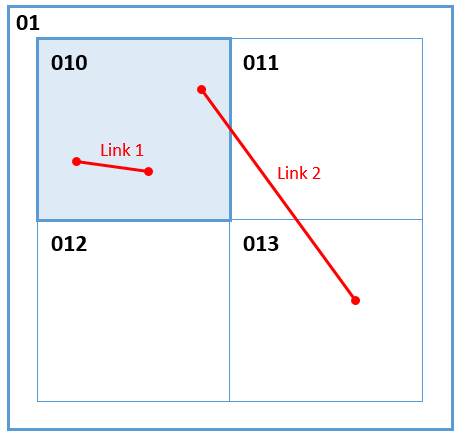
\includegraphics[height=9cm]{images/QuadTile_example.PNG}
\caption{Beispiel QuadTile}
QuadKey Link 1: 010\\QuadKey Link 2: 01
\label{pic:example_quadtile}
\end{figure}
\noindent
\subsection{MinLevel}
Zusätzlich zu dem QuadKey wird beim Import noch für jeden Link der Mindest-Level (MinLevel) berechnet. Denn nur mit dem QuadKey würden alle Strassen in der aktuell angezeigten Bounding Box geladen werden. Auch die eher kleineren Nebenstrassen. Aus diesem Grund setzen wir beim Import ein MinLevel. Dieser MinLevel sagt aus, ab welchem Zoom Level in der Map diese Strasse geladen wird.\\
Der MinLevel einer Strasse wird wie folgt berechnet:\\[0.3cm]
\begin{tabular}{l c l} 
Level 10 & => & Geschwindigkeit > 30 m/s und Anzahl Spuren > 2 \\ 
Level 11 & => & Geschwindigkeit > 30 m/s  \\ 
Level 12 & => & Geschwindigkeit > 23 m/s \\ 
Level 13 & => & Geschwindigkeit > 14 m/s \\ 
Level 14 & => & Geschwindigkeit > 13 m/s und Kapazität >= 4000  \\ 
Level 15 & => & Geschwindigkeit > 13 m/s \\ 
Level 16 & => & Der Rest \\ 
\end{tabular} 
\section{Performance Optimierungen}
Die Performance ist ein sehr wichtiger Faktor in dieser Arbeit. Ohne starke Performance kann die grosse Datenmenge in diesem Projekt nicht effizient dargestellt werden. Dies führte dazu, dass einiges an Zeit in die Performance Optimierung investiert wurde.
\subsection{Caching}
Für die Anzeige der Strassen und Nodes werden sehr viele Daten übertragen. Damit die Daten bei mehrmaligem anfragen nicht jedes Mal übertragen werden müssen, wird sowohl Client seitiges als auch Server seitiges Caching verwendet.\\

TODO
\subsection{Neuzeichnung der Daten verhindern}
TODO
\subsection{Datenbank Index \& Redundanz}
TODO
\section{Infrastruktur}
TODO
\subsection{Docker}
TODO
\subsection{Load Balancing}
TODO
